\documentclass{ximera}

 

\usepackage{epsfig}

\graphicspath{
  {./}
  {figures/}
}

\usepackage{morewrites}
\makeatletter
\newcommand\subfile[1]{%
\renewcommand{\input}[1]{}%
\begingroup\skip@preamble\otherinput{#1}\endgroup\par\vspace{\topsep}
\let\input\otherinput}
\makeatother

\newcommand{\includeexercises}{\directlua{dofile("/home/jim/linearAlgebra/laode/exercises.lua")}}

%\newcounter{ccounter}
%\setcounter{ccounter}{1}
%\newcommand{\Chapter}[1]{\setcounter{chapter}{\arabic{ccounter}}\chapter{#1}\addtocounter{ccounter}{1}}

%\newcommand{\section}[1]{\section{#1}\setcounter{thm}{0}\setcounter{equation}{0}}

%\renewcommand{\theequation}{\arabic{chapter}.\arabic{section}.\arabic{equation}}
%\renewcommand{\thefigure}{\arabic{chapter}.\arabic{figure}}
%\renewcommand{\thetable}{\arabic{chapter}.\arabic{table}}

%\newcommand{\Sec}[2]{\section{#1}\markright{\arabic{ccounter}.\arabic{section}.#2}\setcounter{equation}{0}\setcounter{thm}{0}\setcounter{figure}{0}}

\newcommand{\Sec}[2]{\section{#1}}

\setcounter{secnumdepth}{2}
%\setcounter{secnumdepth}{1} 

%\newcounter{THM}
%\renewcommand{\theTHM}{\arabic{chapter}.\arabic{section}}

\newcommand{\trademark}{{R\!\!\!\!\!\bigcirc}}
%\newtheorem{exercise}{}

\newcommand{\dfield}{{\sf dfield9}}
\newcommand{\pplane}{{\sf pplane9}}

\newcommand{\EXER}{\section*{Exercises}}%\vspace*{0.2in}\hrule\small\setcounter{exercise}{0}}
\newcommand{\CEXER}{}%\vspace{0.08in}\begin{center}Computer Exercises\end{center}}
\newcommand{\TEXER}{} %\vspace{0.08in}\begin{center}Hand Exercises\end{center}}
\newcommand{\AEXER}{} %\vspace{0.08in}\begin{center}Hand Exercises\end{center}}

% BADBAD: \newcommand{\Bbb}{\bf}

\newcommand{\R}{\mbox{$\Bbb{R}$}}
\newcommand{\C}{\mbox{$\Bbb{C}$}}
\newcommand{\Z}{\mbox{$\Bbb{Z}$}}
\newcommand{\N}{\mbox{$\Bbb{N}$}}
\newcommand{\D}{\mbox{{\bf D}}}
\usepackage{amssymb}
%\newcommand{\qed}{\hfill\mbox{\raggedright$\square$} \vspace{1ex}}
%\newcommand{\proof}{\noindent {\bf Proof:} \hspace{0.1in}}

\newcommand{\setmin}{\;\mbox{--}\;}
\newcommand{\Matlab}{{M\small{AT\-LAB}} }
\newcommand{\Matlabp}{{M\small{AT\-LAB}}}
\newcommand{\computer}{\Matlab Instructions}
\newcommand{\half}{\mbox{$\frac{1}{2}$}}
\newcommand{\compose}{\raisebox{.15ex}{\mbox{{\scriptsize$\circ$}}}}
\newcommand{\AND}{\quad\mbox{and}\quad}
\newcommand{\vect}[2]{\left(\begin{array}{c} #1_1 \\ \vdots \\
 #1_{#2}\end{array}\right)}
\newcommand{\mattwo}[4]{\left(\begin{array}{rr} #1 & #2\\ #3
&#4\end{array}\right)}
\newcommand{\mattwoc}[4]{\left(\begin{array}{cc} #1 & #2\\ #3
&#4\end{array}\right)}
\newcommand{\vectwo}[2]{\left(\begin{array}{r} #1 \\ #2\end{array}\right)}
\newcommand{\vectwoc}[2]{\left(\begin{array}{c} #1 \\ #2\end{array}\right)}

\newcommand{\ignore}[1]{}


\newcommand{\inv}{^{-1}}
\newcommand{\CC}{{\cal C}}
\newcommand{\CCone}{\CC^1}
\newcommand{\Span}{{\rm span}}
\newcommand{\rank}{{\rm rank}}
\newcommand{\trace}{{\rm tr}}
\newcommand{\RE}{{\rm Re}}
\newcommand{\IM}{{\rm Im}}
\newcommand{\nulls}{{\rm null\;space}}

\newcommand{\dps}{\displaystyle}
\newcommand{\arraystart}{\renewcommand{\arraystretch}{1.8}}
\newcommand{\arrayfinish}{\renewcommand{\arraystretch}{1.2}}
\newcommand{\Start}[1]{\vspace{0.08in}\noindent {\bf Section~\ref{#1}}}
\newcommand{\exer}[1]{\noindent {\bf \ref{#1}}}
\newcommand{\ans}{}
\newcommand{\matthree}[9]{\left(\begin{array}{rrr} #1 & #2 & #3 \\ #4 & #5 & #6
\\ #7 & #8 & #9\end{array}\right)}
\newcommand{\cvectwo}[2]{\left(\begin{array}{c} #1 \\ #2\end{array}\right)}
\newcommand{\cmatthree}[9]{\left(\begin{array}{ccc} #1 & #2 & #3 \\ #4 & #5 &
#6 \\ #7 & #8 & #9\end{array}\right)}
\newcommand{\vecthree}[3]{\left(\begin{array}{r} #1 \\ #2 \\
#3\end{array}\right)}
\newcommand{\cvecthree}[3]{\left(\begin{array}{c} #1 \\ #2 \\
#3\end{array}\right)}
\newcommand{\cmattwo}[4]{\left(\begin{array}{cc} #1 & #2\\ #3
&#4\end{array}\right)}

\newcommand{\Matrix}[1]{\ensuremath{\left(\begin{array}{rrrrrrrrrrrrrrrrrr} #1 \end{array}\right)}}

\newcommand{\Matrixc}[1]{\ensuremath{\left(\begin{array}{cccccccccccc} #1 \end{array}\right)}}



\renewcommand{\labelenumi}{\theenumi)}
\newenvironment{enumeratea}%
{\begingroup
 \renewcommand{\theenumi}{\alph{enumi}}
 \renewcommand{\labelenumi}{(\theenumi)}
 \begin{enumerate}}
 {\end{enumerate}\endgroup}



\newcounter{help}
\renewcommand{\thehelp}{\thesection.\arabic{equation}}

%\newenvironment{equation*}%
%{\renewcommand\endequation{\eqno (\theequation)* $$}%
%   \begin{equation}}%
%   {\end{equation}\renewcommand\endequation{\eqno \@eqnnum
%$$\global\@ignoretrue}}

%\input{psfig.tex}

\author{Martin Golubitsky and Michael Dellnitz}

%\newenvironment{matlabEquation}%
%{\renewcommand\endequation{\eqno (\theequation*) $$}%
%   \begin{equation}}%
%   {\end{equation}\renewcommand\endequation{\eqno \@eqnnum
% $$\global\@ignoretrue}}

\newcommand{\soln}{\textbf{Solution:} }
\newcommand{\exercap}[1]{\centerline{Figure~\ref{#1}}}
\newcommand{\exercaptwo}[1]{\centerline{Figure~\ref{#1}a\hspace{2.1in}
Figure~\ref{#1}b}}
\newcommand{\exercapthree}[1]{\centerline{Figure~\ref{#1}a\hspace{1.2in}
Figure~\ref{#1}b\hspace{1.2in}Figure~\ref{#1}c}}
\newcommand{\para}{\hspace{0.4in}}

\renewenvironment{solution}{\suppress}{\endsuppress}

\ifxake
\newenvironment{matlabEquation}{\begin{equation}}{\end{equation}}
\else
\newenvironment{matlabEquation}%
{\let\oldtheequation\theequation\renewcommand{\theequation}{\oldtheequation*}\begin{equation}}%
  {\end{equation}\let\theequation\oldtheequation}
\fi

\makeatother


\title{Determinants}

\begin{document}
\begin{abstract}
\end{abstract}
\maketitle

 
\label{S:det}
 
There are several equivalent ways to introduce determinants --- none of which 
are easily motivated.  We prefer to define determinants through the properties 
they satisfy rather than by formula.  These properties actually enable us to 
compute determinants of $n\times n$ matrices where $n>3$, which further 
justifies the approach. Later on, we will give an inductive formula 
\Ref{e:inductdet} for computing the determinant. 
 
\begin{Def}  \label{D:determinants}
A {\em determinant\/} of a square $n\times n$ matrix $A$ is a real
number that satisfies the following three properties:
\begin{itemize} 
\item[(a)]  If $A=(a_{ij})$ is lower 
triangular\index{matrix!lower triangular}, then
the determinant of $A$ is the product of the diagonal entries;
that is,
\[
\det(A) = a_{11}\cdot\cdots\cdot a_{nn}.
\]
\item[(b)]  $\det(A^t)=\det(A)$\index{matrix!transpose}.
\item[(c)]  Let $B$ be an $n\times n$ matrix.  
Then
\begin{equation} \label{e:detproduct}
\det(AB) = \det(A)\det(B).
\end{equation}
\end{itemize}
\end{Def} \index{determinant}

\begin{thm}  \label{T:determinants}
There exists a unique determinant function satisfying the three
properties of Definition~\ref{D:determinants}.
\end{thm}\index{determinant!uniqueness}

We will show that it is possible to compute the determinant of
any $n\times n$ matrix using Definition~\ref{D:determinants}.
Here we present a few examples:

\begin{lemma}
Let $A$ be an $n\times n$ matrix.
\begin{itemize}
\item[(a)]   Let $c\in\R$ be a scalar.  Then $\det(cA) = c^n\det(A)$.
\item[(b)] If all of the entries in either a row or a column of $A$ are 
zero, then $\det(A)=0$.
\end{itemize}
\end{lemma}

\begin{proof}  (a) Note that Definition~\ref{D:determinants}(a) implies that 
$\det(cI_n)=c^n$.  It follows from \Ref{e:detproduct} that
\[
\det(cA) = \det(cI_n A) = \det(cI_n)\det(A) = c^n\det(A).
\]

(b)  Definition~\ref{D:determinants}(b) implies that it suffices to prove 
this assertion when one row of $A$ is zero.  Suppose that the $i^{th}$ row 
of $A$ is zero.  Let $J$ be an $n\times n$ 
diagonal matrix with a $1$ in every diagonal entry except the $i^{th}$ 
diagonal entry which is $0$.  A matrix calculation shows that $JA=A$. 
It follows from Definition~\ref{D:determinants}(a) that $\det(J)=0$ and 
from \Ref{e:detproduct} that $\det(A)=0$.  \end{proof} 



\subsection*{Determinants of $2\times 2$ Matrices}
\index{determinant!of $2\times 2$ matrices} 
 
Before discussing how to compute determinants, we discuss the
special case of $2\times 2$ matrices.  Recall from \Ref{D:determinant} of 
Section~\ref{S:det2x2} that when 
\[
A=\left(\begin{array}{cc} a & b\\c & d \end{array}\right)
\]
we defined 
\begin{equation}  \label{e:determinantn=2}
\det(A)=ad-bc.
\end{equation}
We check that \Ref{e:determinantn=2} satisfies the three
properties in Definition~\ref{D:determinants}.  Observe that when
$A$ is lower triangular, then $b=0$ and $\det(A)=ad$.  So (a) is
satisfied.  It is straightforward to verify (b).  We already
verified (c) in Chapter~\ref{chap:matrices}, Proposition~\ref{propdet}.

It is less obvious perhaps --- but true nonetheless --- that the
three properties of $\det(A)$ actually force the determinant of
$2\times 2$ matrices to be given by formula
\Ref{e:determinantn=2}. We begin by showing that
Definition~\ref{D:determinants} implies that 
\begin{equation}  \label{e:detswap}
\det \left(\begin{array}{cc} 0 & 1\\1 & 0 \end{array}\right)=-1.
\end{equation}
We verify this by observing that 
\begin{equation} \label{e:swapdecomp}
\left(\begin{array}{cc} 0 & 1\\1 & 0 \end{array}\right) =
\left(\begin{array}{cr} 1 & -1\\0 & 1 \end{array}\right)
\left(\begin{array}{cc} 1 & 0\\1 & 1 \end{array}\right)
\left(\begin{array}{cr} 1 & 0\\0 & -1 \end{array}\right)
\left(\begin{array}{cc} 1 & 1\\0 & 1 \end{array}\right).
\end{equation}
Hence property (c), (a) and (b) imply that
\[
\det \left(\begin{array}{cc} 0 & 1\\1 & 0 \end{array}\right) =
1\cdot 1\cdot (-1) \cdot 1 = -1.
\]
It is helpful to interpret the matrices in \Ref{e:swapdecomp} as
elementary row operations\index{elementary row operations}.  
Then \Ref{e:swapdecomp} states that
swapping two rows in a $2\times 2$ matrix is the same as
performing the following row operations in order:
\begin{itemize}
\item        add the $2^{nd}$ row to the  $1^{st}$ row;
\item        multiply the $2^{nd}$ row by $-1$; 
\item        add the $1^{st}$ row to the $2^{nd}$ row; and  
\item        subtract the $2^{nd}$ row from the $1^{st}$ row.
\end{itemize}
 
Suppose that $d\neq 0$.  Then 
\[
A=\left(\begin{array}{cc} a & b\\c & d \end{array}\right) =
\left(\begin{array}{cc} 1 & \frac{b}{d}\\0 & 1 \end{array}\right)
\left(\begin{array}{cc} \frac{ad-bc}{d} & 0\\c & d
\end{array}\right). 
\]
It follows from properties (c), (b) and (a) that
\[
\det(A) = \frac{ad-bc}{d}d = ad-bc,
\]
as claimed.
 
Now suppose that $d=0$ and note that 
\[
A=\left(\begin{array}{cc} a & b\\c & 0 \end{array}\right) = 
\left(\begin{array}{cc} 0 & 1\\1 & 0 \end{array}\right)
\left(\begin{array}{cc} c & 0\\a & b \end{array}\right).
\]
Using \Ref{e:detswap} we see that 
\[
\det(A) = -\det \left(\begin{array}{cc} c & 0\\a & b
\end{array}\right) = -bc,
\]
as desired. 
 
We have verified that the only possible determinant function for
$2\times 2$ matrices is the determinant function defined by
\Ref{e:determinantn=2}. 
 



\subsection*{Row Operations are Invertible Matrices} 
\index{elementary row operations}

\begin{prop}  \label{P:ERO}
Let $A$ and $B$ be $m\times n$ matrices where $B$ is obtained from $A$ by
a single elementary row operation.  Then there exists an invertible 
$m\times m$ matrix $R$ such that $B=RA$.
\end{prop} 

\begin{proof}  First consider multiplying the $j^{th}$ row of $A$ by the
nonzero constant $c$.  Let $R$ be the diagonal matrix whose
$j^{th}$ entry on the diagonal is $c$ and whose other diagonal 
entries are $1$.  Then the matrix $RA$ is just the matrix obtained from 
$A$ by multiplying the $j^{th}$ row of $A$ by $c$.  Note that $R$ is
invertible when $c\neq 0$ and that $R\inv$ is the diagonal
matrix whose $j^{th}$ entry is $\frac{1}{c}$ and whose other
diagonal entries are $1$.  For example
\[
\left(\begin{array}{ccc} 1 & 0 & 0\\ 0 & 1 & 0 \\ 0 & 0 & 2\end{array}\right)
\left(\begin{array}{ccc} a_{11} & a_{12} & a_{13}\\ a_{21} & a_{22} & a_{23}
 \\ a_{31} & a_{32} & a_{33} \end{array}\right) =
\left(\begin{array}{ccc} a_{11} & a_{12} & a_{13}\\ a_{21} & a_{22} & a_{23}
 \\ 2a_{31} & 2a_{32} & 2a_{33} \end{array}\right),
\]
multiplies the $3^{rd}$ row by $2$.

Next we show that the elementary row operation that swaps two
rows may also be thought of as matrix multiplication.  Let
$R=(r_{kl})$ be the matrix that deviates from the identity matrix
by changing in the four entries:
\begin{eqnarray*}
r_{ii} & = & 0 \\
r_{jj} & = & 0\\
r_{ij} & = & 1 \\
r_{ji} & = & 1
\end{eqnarray*}
A calculation shows that $RA$ is the matrix obtained from $A$ by
swapping the $i^{th}$ and $j^{th}$ rows.  For example,
\[
\left(\begin{array}{ccc} 0 & 0 & 1\\ 0 & 1 & 0 \\ 1 & 0 & 0\end{array}\right)
\left(\begin{array}{ccc} a_{11} & a_{12} & a_{13}\\ a_{21} & a_{22} & a_{23}
 \\ a_{31} & a_{32} & a_{33} \end{array}\right) =
\left(\begin{array}{ccc} a_{31} & a_{32} & a_{33}\\ a_{21} & a_{22} & a_{23}
 \\  a_{11} & a_{12} & a_{13} \end{array}\right),
\]
which swaps the $1^{st}$ and $3^{rd}$ rows.  Another calculation
shows that $R^2=I_n$ and hence that $R$ is invertible since
$R\inv=R$.  

Finally, we claim that adding $c$ times the $i^{th}$ row of $A$
to the $j^{th}$ row of $A$ can be viewed as matrix
multiplication.  Let $E_{k\ell}$ be the matrix all of whose
entries are $0$ except for the entry in the $k^{th}$ row and
$\ell^{th}$ column which is $1$.  Then $R=I_n+cE_{ij}$ has the
property that $RA$ is the matrix obtained by adding $c$ times
the $j^{th}$ row of $A$ to the $i^{th}$ row.  We can verify by
multiplication that $R$ is invertible and that
$R\inv=I_n-cE_{ij}$.  More precisely,
\[
(I_n+cE_{ij})(I_n-cE_{ij})=I_n+cE_{ij}-cE_{ij}-c^2E_{ij}^2=I_n,
\]
since $E_{ij}^2 = O$ for $i\not= j$.  For example,
\begin{eqnarray*}
(I_3 + 5E_{12})A &  = & \left(\begin{array}{ccc} 1 & 5 & 0\\ 0 & 1 & 0 \\ 0 & 0 & 1\end{array}\right)
\left(\begin{array}{ccc} a_{11} & a_{12} & a_{13}\\ a_{21} & a_{22} & a_{23}
 \\ a_{31} & a_{32} & a_{33} \end{array}\right) \\ & = & 
\left(\begin{array}{ccc} a_{11}+5a_{21} & a_{12}+5a_{22} & a_{13}+5a_{23} \\ 
a_{21} & a_{22} & a_{23} \\ a_{31} & a_{32} & a_{33} \end{array}\right),
\end{eqnarray*}
adds $5$ times the $2^{nd}$ row to the $1^{st}$ row.   \end{proof}

\subsubsection*{Determinants of Elementary Row Matrices}

\begin{lemma}  \label{L:detelemrowmat}
\begin{itemize}
\item[(a)] The determinant of a swap matrix is $-1$.
\item[(b)] The determinant of the matrix that adds a multiple
of one row to another is $1$.
\item[(c)] The determinant of the matrix that multiplies one
row by $c$ is $c$.
\end{itemize}
\end{lemma}  \index{determinant}
 
\begin{proof} The matrix that swaps the $i^{th}$ row with the $j^{th}$
row is the matrix whose nonzero elements are $a_{kk}=1$ where
$k\neq i,j$ and $a_{ij}=1=a_{ji}$.  Using a similar argument as
in \Ref{e:detswap} we see that the determinants of these
matrices are equal to $-1$.
 
The matrix that adds a multiple of one row to another is
triangular (either upper or lower) and has $1$'s on the
diagonal.  Thus property (a) in Definition~\ref{D:determinants}
implies that the determinants of
these matrices are equal to $1$.
 
Finally, the matrix that multiplies the $i^{th}$ row by $c\neq
0$ is a diagonal matrix all of whose diagonal entries are $1$
except for $a_{ii}=c$.  Again property (a) implies that the
determinant of this matrix is $c\neq 0$. \end{proof}


\subsection*{Computation of Determinants}
\index{determinant!computation}

We now show how to compute the determinant of any $n\times n$ matrix $A$ 
using elementary row operations and Definition~\ref{D:determinants}.  It 
follows from Proposition~\ref{P:ERO} that every elementary row operation 
on $A$ may be performed by premultiplying $A$ by an elementary row matrix. 

For each matrix $A$ there is a unique 
reduced echelon form\index{echelon form!reduced} matrix
$E$ and a sequence of elementary row matrices $R_1\ldots R_s$
such that \index{elementary row operations}
\begin{equation}  \label{e:rowreduction}
E = R_s\cdots R_1A.
\end{equation}
It follows from Definition~\ref{D:determinants}(c) that we can
compute the determinant of $A$ once we know the determinants of
reduced echelon form matrices and the determinants of elementary
row matrices.  In particular
\begin{equation}  \label{e:detformula}
\det(A) = \det(E)/(\det(R_1)\cdots\det(R_s)).
\end{equation}

It is easy to compute the determinant of any matrix in reduced echelon 
form using Definition~\ref{D:determinants}(a) since all reduced echelon 
form $n\times n$ matrices are upper triangular.  Lemma~\ref{L:detelemrowmat}  
tells us how to compute the determinants of elementary row matrices.  This 
discussion proves: 
\begin{prop}
If a determinant function exists for $n\times n$ matrices, then it is unique. 
\index{determinant!uniqueness}
\end{prop}

We still need to show that determinant functions exist when $n>2$.  More 
precisely, we know that the reduced echelon form matrix $E$ is uniquely 
defined from $A$ (Chapter~\ref{lineq}, Theorem~\ref{uniquerowechelon}), but 
there is more than one way to perform elementary row operations on $A$ to 
get to $E$.  Thus, we can write $A$ in the form \Ref{e:detformula} in many 
different ways, and these different decompositions might lead to different 
values for $\det A$.  (They don't.)

\subsubsection*{An Example of Determinants by Row Reduction}
\index{row!reduction}

As a practical matter we row reduce a square matrix $A$ by 
premultiplying $A$ by an elementary row matrix $R_j$.  Thus 
\begin{equation} \label{e:pracdet}
\det(A) = \frac{1}{\det(R_j)} \det (R_j A).
\end{equation}
We use this approach to compute the determinant of the 
$4\times 4$ matrix 
\[
A = \left(\begin{array}{rrrr} 0 & 2 & 10 & -2 \\ 1 & 2 & 4 & 0\\
1 & 6 & 1 & -2 \\ 2 & 1 & 1 & 0 \end{array}\right).
\]
The idea is to use \Ref{e:pracdet} to keep track of the 
determinant while row reducing $A$ to upper triangular form. 
For instance, swapping rows changes the sign of the determinant; 
so
\[
\det(A) = -\det\left(\begin{array}{rrrr} 1 & 2 & 4 & 0\\ 0 & 2 & 10 & -2 \\
1 & 6 & 1 & -2 \\ 2 & 1 & 1 & 0 \end{array}\right).
\]
Adding multiples of one row to another leaves the determinant
unchanged; so
\[
\det(A) = -\det\left(\begin{array}{rrrr} 1 & 2 & 4 & 0\\ 0 & 2 & 10 & -2 \\
0 & 4 & -3 & -2 \\ 0 & -3 & -7 & 0 \end{array}\right).
\]
Multiplying a row by a scalar $c$ corresponds to an elementary 
row matrix whose determinant is $c$.  To make sure that we do not 
change the value of $\det(A)$, we have to divide the determinant by 
$c$ as we multiply a row of $A$ by $c$. So as we divide the second 
row of the matrix by $2$, we multiply the whole result by $2$, obtaining   
\[
\det(A) = -2\det\left(\begin{array}{rrrr} 1 & 2 & 4 & 0\\ 0 & 1 & 5 & -1 \\
0 & 4 & -3 & -2 \\ 0 & -3 & -7 & 0 \end{array}\right).
\] 
We continue row reduction by zeroing out the last two entries in
the $2^{nd}$ column, obtaining
\[
\det(A) = -2\det\left(\begin{array}{rrrr} 1 & 2 & 4 & 0\\ 0 & 1 & 5 & -1 \\
0 & 0 & -23 & 2 \\ 0 & 0 & 8 & -3 \end{array}\right)
= 46\det\left(\begin{array}{rrrr} 1 & 2 & 4 & 0\\ 0 & 1 & 5 & -1 \\
0 & 0 & 1 & -\frac{2}{23} \\ 0 & 0 & 8 & -3 \end{array}\right).
\] 
Thus
\[
\det(A) = 46\det\left(\begin{array}{rrrr} 1 & 2 & 4 & 0\\ 0 & 1 & 5 & -1 \\
0 & 0 & 1 & -\frac{2}{23} \\ 0 & 0 & 0 & -\frac{53}{23} \end{array}\right)
= -106.
\]  

\subsubsection*{Determinants and Inverses}
\index{inverse}

We end this subsection with an important observation about the
determinant function.  This observation generalizes to dimension
$n$ Corollary~\ref{C:2x2invert} of Chapter~\ref{chap:matrices}. 
\begin{thm}  \label{T:detandinv}
An $n\times n$ matrix $A$ is invertible if and only if $\det(A)\neq 0$.
Moreover, if $A\inv$ exists, then 
\begin{equation}  \label{E:detinv}
\det A\inv = \frac{1}{\det A}.
\end{equation}
\end{thm} \index{invertible}
 
\begin{proof}  If $A$ is invertible, then 
\[
\det(A)\det(A\inv) = \det(AA\inv) = \det(I_n) =1.
\]
Thus $\det(A)\neq 0$ and \Ref{E:detinv} is valid. In particular, the 
determinants of elementary row matrices are nonzero, since they are all
invertible. (This point was proved by direct calculation in
Lemma~\ref{L:detelemrowmat}.)
 
If $A$ is singular, then $A$ is row equivalent to a non-identity
reduced echelon form matrix $E$ whose determinant is zero (since
$E$ is upper triangular and its last diagonal entry is zero).
So it follows from
\Ref{e:rowreduction} that 
\[
0=\det(E) = \det(R_1)\cdots\det(R_s)\det(A)
\]
Since $\det(R_j)\neq 0$, it follows that $\det(A)=0$.  \end{proof}

\begin{cor}
If the rows of an $n\times n$ matrix $A$ are linearly dependent (for example,
if one row of $A$ is a scalar multiple of another row of $A$), then 
$\det(A)=0$.
\end{cor}


\subsection*{An Inductive Formula for Determinants} 
\index{determinant!inductive formula for}
 
In this subsection we present an inductive formula for the
determinant --- that is, we assume that the determinant is known
for square $(n-1)\times(n-1)$ matrices and use this formula to
define the determinant for $n\times n$ matrices.  This inductive formula
is called {\em expansion by cofactors\/}.
 
Let $A=(a_{ij})$ be an $n\times n$ matrix.  Let $A_{ij}$ be the
$(n-1)\times(n-1)$ matrix formed from $A$ by deleting the
$i^{th}$ row and the $j^{th}$ column.  The matrices $(-1)^{i+j}A_{ij}$ are
called {\em cofactor\/} \index{cofactor} matrices of $A$.  

Inductively we define the determinant of an $n\times n$ matrix $A$ by:
\begin{eqnarray}  
\det(A) & = & \sum^n_{j=1} (-1)^{1+j}a_{1j}\det(A_{1j}) \nonumber
\\  & = &
a_{11}\det(A_{11})-a_{12}\det(A_{12})+\cdots+(-1)^{n+1}a_{1n}\det(A_{1n}).
    \label{e:inductdet}
\end{eqnarray} \index{determinant}
In Appendix~\ref{A:det} we show that the determinant function defined by 
\Ref{e:inductdet} satisfies all properties of a determinant function.
Formula \Ref{e:inductdet} is also called {\em expansion by cofactors along 
the $1^{st}$ row\/}, since the $a_{1j}$ are taken from the $1^{st}$ row 
of $A$.  Since $\det(A)=\det(A^t)$, it follows that if \Ref{e:inductdet} is 
valid as an inductive definition of determinant, then expansion by cofactors 
along the $1^{st}$ column is also valid.  That is,
\begin{equation}  \label{e:inductdetc}
\det(A) = 
a_{11}\det(A_{11})-a_{21}\det(A_{21})+\cdots+(-1)^{n+1}a_{n1}\det(A_{n1}).
\end{equation} 

We now explore some of the consequences of this definition, beginning 
with determinants of small matrices.  For example, 
Definition~\ref{D:determinants}(a) implies that the determinant of a 
$1\times 1$ matrix is just
\[
\det(a) = a.
\]
Therefore, using \Ref{e:inductdet}, the determinant of a $2\times
2$ matrix is:
\[
\det\left(\begin{array}{cc} a_{11} & a_{12}\\a_{21} & a_{22}
\end{array}\right) = a_{11}\det(a_{22}) - a_{12}\det(a_{21}) =
a_{11}a_{22} - a_{12}a_{21},
\]
which is just the formula for determinants of $2\times 2$
\index{determinant!of $2\times 2$ matrices}
matrices given in \Ref{e:determinantn=2}. 
 
Similarly, we can now find a formula for the determinant of
$3\times 3$ matrices $A$ as follows.
\begin{eqnarray} 
\det(A) & = & a_{11}
\det \left(\begin{array}{cc} a_{22} & a_{23}\\a_{32} & a_{33}
\end{array}\right) 
- a_{12}
\det \left(\begin{array}{cc} a_{21} & a_{23}\\a_{31} & a_{33}
\end{array}\right) 
+ a_{13}
\det\left(\begin{array}{cc} a_{21} & a_{22}\\a_{31} & a_{32}
\end{array}\right) \nonumber \\
 & & \label{e:det3} \\
& = & a_{11}a_{22}a_{33} + a_{12}a_{23}a_{31} + a_{13}a_{21}a_{32}
- a_{11}a_{23}a_{32} - a_{12}a_{21}a_{33} - a_{13}a_{22}a_{31}. \nonumber
\end{eqnarray}  

As an example, compute
\[
\det\left(\begin{array}{rrr} 2 & 1 & 4\\ 1 & -1 & 3\\ 5 & 6 & -2
\end{array}\right) 
\]
using formula \Ref{e:det3} as
\[
2(-1)(-2) + 1\cdot3\cdot5 + 4\cdot6\cdot1 -4(-1)5 -3\cdot6\cdot2
- (-2)1\cdot1  = 4+15+24+20 -36 +2 = 29. 
\]

There is a visual mnemonic for remembering how to compute the six
terms in formula \Ref{e:det3} for the determinant of 
$3\times 3$ matrices\index{determinant!of $3\times 3$ matrices}.
Write the matrix as a $3\times 5$ array by repeating the first 
two columns, as shown in bold face in Figure~\ref{F:det3}:
\index{determinant!computation}
\begin{figure}[htb]
           \centerline{%
            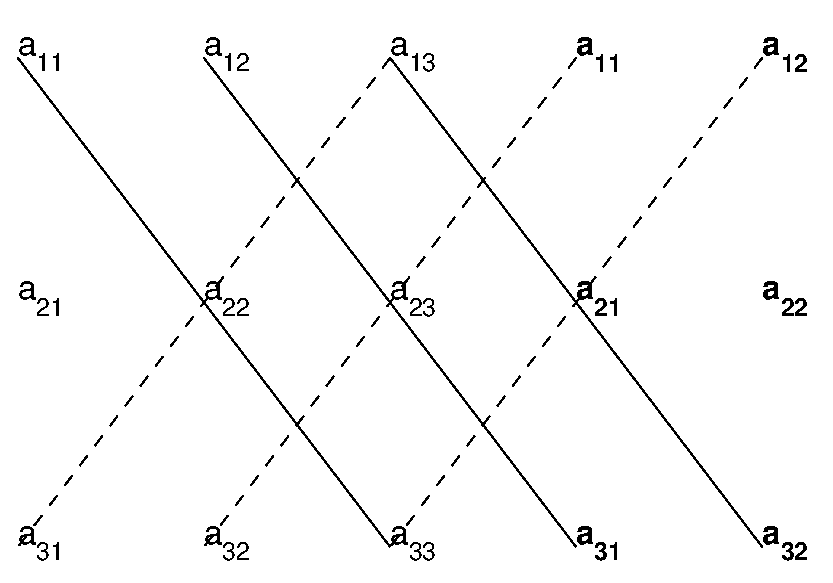
\psfig{file=figures/det3.eps,height=2.5in}}
           \caption{Mnemonic for computation of determinants of 
		$3\times 3$ matrices.}
           \label{F:det3}
\end{figure}
Then add the product of terms connected by solid lines sloping down and 
to the right and subtract the products of terms connected by dashed lines 
sloping up and to the right.  Warning: this nice crisscross algorithm 
for computing determinants of $3\times 3$ matrices does not generalize 
to $n\times n$ matrices.
 
When computing determinants of $n\times n$ matrices when $n>3$,
it is usually more efficient to compute the determinant using row
reduction rather than by using formula \Ref{e:inductdet}.  In the
appendix to this chapter, Section~\ref{A:det}, we verify that formula 
\Ref{e:inductdet} actually satisfies the three properties of a determinant, 
thus completing the proof of Theorem~\ref{T:determinants}.  

An interesting and useful formula for reducing the effort in 
computing determinants is given by the following formula.
\begin{lemma} \label{L:detblockdiag}
Let $A$ be an $n\times n$ matrix of the form
\[
A=\mattwo{B}{0}{C}{D},
\]
where $B$ is a $k\times k$ matrix and $D$ is an $(n-k)\times(n-k)$
matrix.  Then
\[
\det(A)=\det(B)\det(D).
\]
\end{lemma}

\begin{proof} We prove this result using \Ref{e:inductdet} coupled with 
induction. Assume that this lemma is valid or all $(n-1)\times
(n-1)$ matrices of the appropriate form.  Now use
\Ref{e:inductdet} to compute
\begin{eqnarray*}
\det(A) & = & a_{11}\det(A_{11})-a_{12}\det(A_{12}) + \cdots\pm
a_{1n}\det(A_{1n}) \\
& = &  b_{11}\det(A_{11})-b_{12}\det(A_{12}) + \cdots\pm
b_{1k}\det(A_{1k}).
\end{eqnarray*}
Note that the cofactor matrices $A_{1j}$ are obtained from $A$
by deleting the $1^{st}$ row and the $j^{th}$ column.  These
matrices all have the form
\[
A_{1j} = \mattwo{B_{1j}}{0}{C_j}{D},
\]
where $C_j$ is obtained from $C$ by deleting the $j^{th}$
column. By induction on $k$
\[
\det(A_{1j}) = \det(B_{1j})\det(D).
\]
It follows that 
\begin{eqnarray*}
\det(A) & = & \left(b_{11}\det(B_{11})-b_{12}\det(B_{12}) + \cdots\pm
b_{1k}\det(B_{1k})\right)\det(D) \\
& = & \det(B)\det(D),
\end{eqnarray*}
as desired.  \end{proof}


\subsection*{Determinants in \Matlab}
\index{determinant!in \protect\Matlab}

The determinant function has been preprogrammed in \Matlab and
is quite easy to use.  For example, typing {\tt e8\_1\_11} will
load the matrix
\begin{equation*}  \label{e:A4x4}
A = \left(\begin{array}{rrrr}
     1   &  2  &   3  &   0\\
     2   &  1  &   4  &   1\\
    -2   & -1  &   0  &   1\\
    -1   &  0  &  -2  &   3  \end{array} \right).
\end{equation*}
To compute the determinant of $A$ just type {\tt det(A)} and
obtain the answer \index{\computer!det}
\begin{verbatim}
ans =
   -46
\end{verbatim}

Alternatively, we can use row reduction techniques in \Matlab to
compute the determinant of $A$ --- just to test the theory that
we have developed.  Note that to compute the determinant we do
not need to row reduce to 
reduced echelon form\index{echelon form!reduced} --- we need only
reduce to an upper triangular matrix.  This can always be done
by successively adding multiples of one row to another --- an
operation that does not change the determinant.  For example,
to clear the entries in the $1^{st}$ column below the $1^{st}$
row, type
\begin{verbatim}
A(2,:) = A(2,:) - 2*A(1,:);
A(3,:) = A(3,:) + 2*A(1,:); 
A(4,:) = A(4,:) + A(1,:)
\end{verbatim}
obtaining 
\begin{verbatim}
A =
     1     2     3     0
     0    -3    -2     1
     0     3     6     1
     0     2     1     3
\end{verbatim}
To clear the $2^{nd}$ column below the $2^{nd}$ row type 
\begin{verbatim}
A(3,:) = A(3,:) + A(2,:);A(4,:) = A(4,:) - A(4,2)*A(2,:)/A(2,2)\end{verbatim}
obtaining
\begin{verbatim}
A =
    1.0000    2.0000    3.0000         0
         0   -3.0000   -2.0000    1.0000
         0         0    4.0000    2.0000
         0         0   -0.3333    3.6667
\end{verbatim}
Finally, to clear the entry $(4,3)$ type
\begin{verbatim}
A(4,:) = A(4,:) -A(4,3)*A(3,:)/A(3,3)\end{verbatim}
to obtain
\begin{verbatim}
A =
    1.0000    2.0000    3.0000         0
         0   -3.0000   -2.0000    1.0000
         0         0    4.0000    2.0000
         0         0         0    3.8333
\end{verbatim}
To evaluate the determinant of $A$, which is now an upper
triangular matrix, type
\begin{verbatim}
A(1,1)*A(2,2)*A(3,3)*A(4,4)\end{verbatim}
obtaining
\begin{verbatim}
ans =
   -46
\end{verbatim}
as expected.

\EXER

\TEXER


\noindent  In Exercises~\ref{c10.1.1a} -- \ref{c10.1.1c} compute the 
determinants of the given matrix.
\begin{exercise} \label{c10.1.1a}
$A = \left(\begin{array}{rrr} -2 & 1 & 0 \\ 4 & 5& 0 \\ 1 & 0 & 2
\end{array} \right)$.
\end{exercise} 
\begin{exercise} \label{c10.1.1b}
$B = \left(\begin{array}{rrrr} 1 & 0 & 2 & 3 \\ -1 & -2 & 3 & 2
\\ 4 & -2 & 0 & 3 \\ 1 & 2 & 0 & -3 \end{array} \right)$.
\end{exercise}
\begin{exercise} \label{c10.1.1c}
$C = \left(\begin{array}{rrrrr} 2 & 1 & -1 & 0 & 0 \\ 1 & -2 & 3
& 0 & 0 \\ -3 & 2 & -2 & 0 & 0 \\ 1 & 1 & -1 & 2 & 4 \\ 0 & 2 &
3 & -1 & -3 \end{array} \right)$.
\end{exercise}

\begin{exercise} \label{c10.1.2}
Find $\det(A\inv)$ where 
$A = \left(\begin{array}{rrr} -2 & -3 & 2 \\ 4 & 1 & 3 \\ -1 & 1 & 1
\end{array} \right)$. 
\end{exercise}

\begin{exercise} \label{c10.1.3}
Show that the determinants of similar $n\times n$ matrices are
equal. 
\end{exercise}

\noindent In Exercises~\ref{c10.1.4} -- \ref{c10.1.5b} use row reduction 
to compute the determinant of the given matrix.
\begin{exercise} \label{c10.1.4}
$A = \left(\begin{array}{rrr} -1 & -2 & 1 \\ 3 & 1 & 3 \\ -1 & 1 & 1
\end{array} \right)$. 
\end{exercise}
\begin{exercise} \label{c10.1.5a}
$B = \left(\begin{array}{rrrr} 1 & 0 & 1 & 0 \\ 0 & 1 & 0 & -1 \\
1 & 0 & -1 & 0 \\ 0 & 1 & 0 & 1 \end{array}\right)$.
\end{exercise}
\begin{exercise} \label{c10.1.5b}
$C = \left(\begin{array}{rrrr} 1 & 2 & 0 & 1 \\ 0 & 2 & 1 & 0 \\
-2 & -3 & 3 & -1 \\ 1 & 0 & 5 & 2 \end{array}\right)$.
\end{exercise}

\begin{exercise} \label{c10.1.6}
Let 
\[
A = \left(\begin{array}{rrr} 2 & -1 & 0 \\ 0 & 3 & 0 \\ 1 & 5 & 3
\end{array} \right)  \AND
B = \left(\begin{array}{rrr} 2 & 0 & 0 \\ 0 & -1 & 0 \\ 0 & 0 & 3
\end{array} \right).
\]
\begin{itemize}
\item[(a)] For what values of $\lambda$ is  $\det(\lambda A-B)=0$?
\item[(b)] Is there a vector $x$ for which $Ax=Bx$?
\end{itemize}
\end{exercise}

\noindent In Exercises~\ref{c10.1.a7a} -- \ref{c10.1.a7b} verify 
that the given matrix has determinant $-1$.
\begin{exercise} \label{c10.1.a7a}
$A = \left( \begin{array}{rrr}
1  &  0  &  0\\
0  &  0  &  1\\
0  &  1  &  0
\end{array} \right)$.
\end{exercise}
\begin{exercise} \label{c10.1.a7b}
$B = \left( \begin{array}{rrr}
 0 &   0 &   1\\
 0 &   1 &   0\\
 1 &   0 &   0
\end{array} \right)$.
\end{exercise}


\begin{exercise} \label{c10.1.b7a}
Compute the cofactor matrices $A_{13}, A_{22}, A_{21}$ when 
$A = \left( \begin{array}{rrr}
 3 & 2 & -4\\
 0 & 1 & 5\\
 0 & 0 & 6\end{array} \right)$.
\end{exercise}
\begin{exercise} \label{c10.1.b7b}
Compute the cofactor matrices $B_{11}, B_{23}, B_{43}$ when
$B = \left( \begin{array}{rrrr}
 0 & 2 & -4 & 5\\
 -1 & 7 & -2 & 10\\
 0 & 0 & 0  & -1\\
3 & 4 & 2 & -10
\end{array} \right)$.
\end{exercise}

\begin{exercise} \label{c10.1.c7}
Find values of $\lambda$ where the determinant of the matrix
\[
A_\lambda = \left( \begin{array}{ccr}
 \lambda -1 & 0 & -1\\
 0 & \lambda -1 & 1\\
-1 & 1 & \lambda 
\end{array} \right)
\]
vanishes.  
\end{exercise}

\begin{exercise}  \label{c10.1.c8} 
Suppose that two $n\times p$ matrices $A$ and $B$ are row
equivalent. \index{row!equivalent} Show that there is an invertible
$n\times n$ matrix $P$ such that $B = PA$.
\end{exercise}

\begin{exercise} \label{c10.1.c9}
Let $A$ be an invertible $n\times n$ matrix and let $b\in\R^n$ be a column 
vector. Let $B_j$ be the $n\times n$ matrix obtained from $A$ by replacing the 
$j^{th}$ column of $A$ by the vector $b$.  Let $x=(x_1,\ldots,x_n)^t$ be the 
unique solution to $Ax=b$. Then Cramer's rule \index{Cramer's rule} states that
\begin{equation}  \label{E:cramer2}
x_j = \frac{\det(B_j)}{\det(A)}.
\end{equation}
Prove Cramer's rule.  {\bf Hint}: Let $A_j$ be the $j^{th}$ column of $A$ so
that $A_j = Ae_j$.  Show that 
\[
B_j = A (e_1|\cdots|e_{j-1}|x|e_{j+1}|\cdots|e_n).
\]
Using this product, compute the determinant of $B_j$ and verify \Ref{E:cramer2}.
\end{exercise}

\end{document}
